\documentclass[11pt,a4paper]{article}
\usepackage[margin=24mm]{geometry}
\usepackage{amsmath,amssymb,graphicx,booktabs,adjustbox,placeins,lmodern,microtype}
\usepackage[numbers,sort&compress]{natbib}
\usepackage[hidelinks]{hyperref}
\graphicspath{{figures/}}
\setlength{\emergencystretch}{1em}
\renewcommand{\thesection}{S\arabic{section}}
\renewcommand{\thetable}{S\arabic{table}}
\renewcommand{\thefigure}{S\arabic{figure}}
\title{Supplementary material for\\Evaluating Deadline-Limited Communication in Multi-Agent Reinforcement Learning}
\author{Yeong-woo Kung \quad Young-guk Ha\thanks{Corresponding author. Email: \texttt{ygha@konkuk.ac.kr}.}\\[3pt]
\small Smart Computing Laboratory, Department of Computer Science \& Engineering\\
\small Konkuk University, 120 Neungdong-ro, Gwangjin-gu, Seoul 05029, Republic of Korea\\
\small Yeong-woo Kung: \texttt{yeongwoo@konkuk.ac.kr}\\
\small Young-guk Ha: \texttt{ygha@konkuk.ac.kr}}
\date{}
\begin{document}
\maketitle
\section{Access rules, training and replay}\label{app:settings}
The Hallway and broadcast policies send eight 32-bit floats per packet. Each packet occupies $S=48$ wire bytes including a 16-byte header. For an action deadline $D_{\max}$, the reception cutoff is $D_{\rm recv}=D_{\max}-R_{\rm post}$ with $R_{\rm post}=0.45$ ms reserved for subsequent work. The modeled link has bandwidth $B$ and propagation time $\ell=0.05$ ms. At a receiver, a valid sender entry of age $\tau$ contributes with weight $\lambda^\tau$. An entry persists until that sender's next timely update.

At elapsed admission time $E_t$, the cap combines link capacity and traffic credit:
\begin{align}
 K_{\rm link}(E_t)&=\left\lfloor [D_{\max}-R_{\rm post}-E_t-\ell]_+B/S\right\rfloor,\label{eq:cap}\\
 c_t^-&=\min(c_{\max},c_{t-1}+b),\nonumber\\ K_{\max,t}&=\min\{N,K_{\rm link}(E_t),\lfloor c_t^-/S\rfloor\},\\
 c_t&=c_t^- - SK_t.
\end{align}
Here $b=120$ B/step, $c_{\max}=144$ B and initial credit is zero. This bounds cumulative attempted bytes, not each step's bytes. Candidate packing is charged even if a post-packing cap recheck rejects it. Later bookkeeping can still invalidate an earlier capacity estimate.

Full attempts all senders; Periodic selects $(t+i)\bmod2=0$. RR uses the cap and advances its cursor by the admitted count. DAC uses the same cap but ranks batched local scores
\begin{equation}
 u_i^t=(Q_{i,(1)}^{\rm local}-Q_{i,(2)}^{\rm local})+0.1a_i^{\rm tx,t}.
\end{equation}
The local head has zero communication features; the gap is zero with only one legal action. The threshold is zero and ties use agent ID. Transmitter age starts at zero, resets on an attempt (even if dropped), and increments otherwise. It differs from receiver age. RR/DAC use $\lambda=0.9$; Full/Periodic use $\lambda=1$. Identity controls explicitly match decay. DAC requires all agents' scores at a central scheduler: CPU cost is measured, but physical score-collection traffic is not. Its score is a heuristic, not a measure of marginal receiver utility.
\subsection{Fresh-weight Hallway campaign}
Five agents form groups of sizes two and three. A successful group contributes 10 and both groups can yield a maximum episodic return of 20; the finite horizon is 14 steps. For each of ten seeds, we initialize six configurations from fresh weights: no communication, ideal fresh communication, Full under the modeled channel, Periodic, capacity-capped Round-Robin (RR), and DAC. Each configuration trains for 1,500 updates in each of Slow/5 ms, Medium/2 ms and Medium/5 ms, yielding 180 jobs. Learning uses the Hallway Oracle/BC support specified in this section. This is not demonstration-free learning. Equal update counts do not imply equal environment transition counts, because policies can terminate episodes at different times.

Final checkpoints are evaluated on 50 paired held-out resets in Slow/5 ms, Medium/2 ms, Medium/5 ms and Medium/1.5 ms: 720 seed-level cells and 36,000 episode returns. All seeds remain in primary summaries. There is no best-checkpoint or successful-seed selection. Ideal Full overrides delivery failure to supply fresh messages; it is a reference condition rather than an optimal-return bound. RR uses the same credit, link cap and cache decay as DAC, advances its cursor by admitted sender count, and avoids local-Q priority computation. Equal caps do not imply identical actual bytes when CPU costs or trajectories differ.

\subsection{Statistical and timing controls}
Means and sample SD are computed across independent training seeds. Paired bootstrap resamples seed differences 10,000 times; the BCa sensitivity check uses bias correction and acceleration~\citep{efron1987better}. Episode repetitions do not increase the number of independent training seeds. A supplemental post-hoc exact two-sided sign-flip analysis uses Holm correction~\citep{holm1979simple} separately over three matched-condition Ideal--No-Comm contrasts and the twelve DAC--RR deployment contrasts. Sign-flip inference requires exchangeability under the null, or symmetric paired differences; it is not a distribution-free guarantee. Unadjusted bootstrap intervals and corrected p-values are labeled separately.

CPU evaluation uses one thread, excludes two warmup episodes, disables automatic garbage collection during rollouts and collects outside them. The post-reception reserve is fixed at 0.45 ms. No CPU timing claim is derived from GPU optimization. A separate matched-checkpoint diagnostic fixes preparation time at 0.5 ms for admission and transport while recording actual computation separately. This isolates a common reception opportunity; its virtual timing is not deployable latency.
\paragraph{Primary Hallway learning} Adam~\citep{kingma2015adam} learning rate is $5\times10^{-4}$, discount 0.99, global gradient clip 10, and hard target synchronization every 100 updates. A fresh policy has shared GRU~\citep{cho2014learning} width 64, message width 8 and QMIX mixing~\citep{rashid2018qmix}; Double-Q targets~\citep{hasselt2016deepdouble} use the online network to select the next action and the target network to evaluate that action. The online replay holds 2,000 episodes; 50 Oracle episodes populate a separate demonstration pool. Each 16-episode batch contains 4 demonstration and 12 online episodes, with replacement only while a stratum is too small. One online episode is collected per update; 1,500 updates therefore need not represent equal environment-step counts. The original worker uses exploration $1-0.95u/1499$ at zero-based update $u$. The TD objective adds 0.5 times demonstration cross entropy. Target synchronization and exploration count updates, not environment transitions. All final checkpoints are evaluated, without successful-seed filtering.

\paragraph{Hallway observations and teacher}\label{app:local_clock} Hallway uses the class distributed in the CASEC/MACO code release~\citep{wang2022casec}; the wrapper preserves its reward and transition rules. Each agent observes its own integer distance and active flag. The encoder additionally receives one-hot agent ID and previous action; the mixer state concatenates all distance/active pairs. Distances initialize independently and uniformly in $\{1,2,3,4\}$; group IDs are $[0,0,1,1,1]$. Actions wait, reduce distance by one, or increase distance by one up to four. A group whose members all reach zero together earns 10 and becomes inactive; an asynchronous partial arrival fails that group. If both groups arrive simultaneously, the step first earns +20 and then subtracts 30, giving net reward -10. An episode terminates naturally only when both groups have succeeded or both have failed; mixed success/failure reaches the 14-step horizon. Exact simultaneous-arrival semantics are given in the \emph{Environment aliasing and snapshot isolation} paragraph.

The privileged teacher moves agents toward distance one, then admits the lowest-index ready group. Across all 1,024 starts it obtains return 20; 39 of 120 distinct agent-specific local observation and previous-action history keys map to conflicting teacher actions. This is a count of distinct keys, not a BC error rate or a demonstrated cause of the learned return gap. A different no-message controller moves to distance one and uses public group-specific arrival steps 3 and 4. Given a synchronized reset clock, known roster and maximum initial distance, it obtains return 20 on all 1,024 starts (5,120 steps). This is exhaustive solvability, not neural learning success. BC applies to all agents at filled demonstration timesteps, including inactive agents, but not padding or online episodes.

\paragraph{Environment aliasing and snapshot isolation}
The local variable \texttt{last\_state} aliases the environment's mutable distance array; it is not a saved pre-action copy. During simultaneous two-group arrival, the nominal rollback therefore retains the post-move zero distances. Both group-active flags remain false, agent-active flags are restored true, and the win counter returns to zero. No further group reward is evaluated, and the episode reaches the horizon. This is a preserved task-specific transition rule, not an alias between stored transitions or independent branches. Direct checks verify the net -10 reward and subsequent timeout. Adapter observations and global states are new arrays; episode construction copies them into arrays, replay insertion/sampling deep-copies records, and branch cloning deep-copies mutable environment/harness state while sharing immutable model parameters. Added tests mutate later environment states, replay samples and branch caches and verify the stored/factual data remain unchanged.

\paragraph{Replay consistency} Replay stores full episodes beginning with an empty cache and zero initial recurrent state, not arbitrary chunks. Nonzero initial caches or source timestamps are rejected. The online and target networks each unroll their own recurrent states and regenerate their own messages under current respective parameters. Both use the same recorded delivery events. Consequently, the cache retained between events belongs to that network's latent space; it is not a stale stored vector encoded by older parameters. Next-state bootstrap uses the recorded next-observation delivery event, not a freshly sampled gate. Termination and horizon truncation both suppress bootstrap. This is off-policy evaluation conditional on replayed access history; it is not a claim that current gates would recreate the recorded behavior.

\paragraph{Measurement and artifacts}
Slow and medium links are 20,000 and 100,000 B/s (decimal units). The host is an AMD Ryzen Threadripper 3960X, Python 3.13.12, PyTorch 2.11.0+cu128 and NumPy 2.4.4. Sequential repeat processes use the same allowed CPU, one inference thread, two discarded warmups and automatic GC disabled during rollouts; seed/selector orders are counterbalanced. Identical-input cost checks clone policy, recurrent/cache and scheduler state outside the timer. Fixed readiness replaces preparation time for admission/transport only, while CPU work is separately recorded. These are not extra training seeds or cross-machine replications.

The accompanying evidence archive contains configurations, trained policies, receiver features, paired outcomes and a file-level checksum manifest. The reviewer guide maps each result to its inputs, analysis and validation command. Full-suffix identity tests compare actions, rewards, termination, delivery, cache timestamps and traffic. ``Registered'' refers to configurations recorded before their runs, not public preregistration.
\FloatBarrier
\section{Hallway policy comparisons}
The six separately trained configurations use the same update budget. Table~\ref{tab:primary} reports the matched deployment conditions and two untrained references. Table~\ref{tab:paired} gives the paired contrasts. Figure~\ref{fig:seed_distribution} shows the ten individual seed means.
\begin{table}[htbp]\centering\setlength{\tabcolsep}{3pt}\small
\caption{Primary Hallway results: independently trained configurations, matched training/deployment condition, all ten seeds, mean and sample SD. Learned rows are Oracle-assisted, 1,500 updates per job, with measured CPU readiness and 50 evaluation resets per seed. Reference rows have no training or messages: random actions use ten action-RNG seeds on the same 50 primary resets (8200000--8200049), with SD across RNG means, not training seeds. The local-clock value is verified over all 1,024 initial states. Neither reference uses the link, so its value is repeated across columns.}\label{tab:primary}
\vspace{2.5mm}
\begin{adjustbox}{max width=\linewidth}\begin{tabular}{lrrr}\toprule
Configuration & Slow/5 ms & Medium/2 ms & Medium/5 ms\\\midrule
No-Comm & $3.96\pm2.27$ & $4.00\pm2.38$ & $4.26\pm1.98$\\
Ideal Full & $11.44\pm2.98$ & $12.20\pm3.04$ & $11.54\pm3.22$\\
Full & $6.60\pm3.15$ & $7.70\pm1.81$ & $11.54\pm3.26$\\
Periodic & $6.54\pm3.53$ & $5.66\pm1.99$ & $7.88\pm4.16$\\
RR & $6.12\pm1.69$ & $5.64\pm1.99$ & $7.88\pm2.25$\\
DAC & $4.72\pm3.13$ & $6.38\pm0.82$ & $7.04\pm3.52$\\
\midrule Random actions (reference) & $0.22\pm0.20$ & $0.22\pm0.20$ & $0.22\pm0.20$\\
Constructive local clock (reference) & 20 & 20 & 20\\
\bottomrule\end{tabular}\end{adjustbox}\end{table}
\begin{table}[htbp]\centering\setlength{\tabcolsep}{3pt}\small
\caption{Paired seed effects. CIs are unadjusted percentile bootstrap intervals. Supplemental post-hoc two-sided sign-flip p-values use Holm correction over three utility contrasts or all twelve train/deployment DAC--RR contrasts.}\label{tab:paired}
\vspace{3mm}
\begin{adjustbox}{max width=\linewidth}\begin{tabular}{llrrr}\toprule
Condition & Contrast & Difference & 95\% CI & Holm p\\\midrule
Medium/2 ms & Ideal--No-Comm & +8.20 & [+5.48,+10.64] & 0.0059\\
Medium/5 ms & Ideal--No-Comm & +7.28 & [+4.88,+9.38] & 0.0059\\
Slow/5 ms & Ideal--No-Comm & +7.48 & [+4.92,+9.94] & 0.0059\\
Medium/2 ms & DAC--RR & +0.74 & [-0.96,+1.96] & 1.0000\\
Medium/5 ms & DAC--RR & -0.84 & [-3.02,+1.26] & 1.0000\\
Slow/5 ms & DAC--RR & -1.40 & [-3.06,+0.08] & 1.0000\\
\bottomrule\end{tabular}\end{adjustbox}\end{table}
In contrast, DAC minus RR is $-1.40$, $+0.74$ and $-0.84$ in the same matched conditions, with every paired interval including zero. The intervals leave both positive and negative selection effects plausible. Among cross-condition deployments, Medium/5 ms training followed by Slow/5 ms deployment gives DAC $+2.60$, unadjusted CI $[0.98,4.34]$; its corrected p-value over all twelve selector comparisons is 0.1875. The favorable deployment cell does not survive that multiplicity control.
For the matched Slow/5 ms trained policies, Full offers 240 wire B/step for 32 payload B/step and 80\% waste. Periodic offers 120.14 B/step for the same payload goodput and approximately 60.05\% waste. Both RR and DAC offer 48 B/step, retain 32 payload B/step, and exhibit zero observed drops, but return is 6.12 for RR and 4.72 for DAC. Capacity capping explains the shared communication saving; it cannot uniquely explain DAC's sender selection.

This reduction follows the modeled capacity constraint. At preparation time $P_{\mathrm{ready},t}$, the link permits at most
\begin{equation}
 K_t^{\mathrm{feasible}}=\left\lfloor \frac{B_{\rm link}[D_{\rm recv}-P_{\mathrm{ready},t}-\ell]_+}{S}\right\rfloor
\end{equation}
arrivals of equal-sized packets. Avoiding attempts beyond this bound prevents modeled late packets if preparation accounting remains exact. The saving follows directly from finite service capacity. Later CPU work and timing variability can still invalidate an earlier cap estimate: matched Medium/2 ms DAC has approximately 0.031\% waste. There it offers 92.23 B/step versus RR's 95.46 B/step; the comparison is same-cap, not exactly equal offered load.
\begin{table}[htbp]\centering\setlength{\tabcolsep}{3pt}\footnotesize
\caption{Exploratory sensitivity of DAC--RR seed-level inference. TOST margin is $\pm1$ return, selected after observing earlier results; MDE is an approximate 80\% power sensitivity based on observed paired SD. No confirmatory equivalence claim follows.}\label{tab:sensitivity}
\vspace{3mm}
\begin{adjustbox}{max width=\linewidth}\begin{tabular}{lrrrrr}\toprule
Condition & Difference & t 95\% CI & BCa 95\% CI & TOST p & MDE 80\\\midrule
Slow/5 ms & -1.40 & [-3.29,0.49] & [-3.26,-0.08] & 0.678 & 2.59\\
Medium/2 ms & +0.74 & [-1.11,2.59] & [-1.77,1.78] & 0.379 & 2.54\\
Medium/5 ms & -0.84 & [-3.47,1.79] & [-2.96,1.36] & 0.447 & 3.60\\
\bottomrule\end{tabular}\end{adjustbox}\end{table}
Table~\ref{tab:sensitivity} shows that BCa and t intervals disagree on zero exclusion for Slow/5 ms, demonstrating method sensitivity at ten seeds. No matched condition passes the exploratory $\pm1$ equivalence criterion, evaluated with two one-sided tests~\citep{schuirmann1987comparison}. The intervals are unadjusted and the sensitivity analysis does not replace the multiplicity-controlled primary analysis.
\begin{figure}[htbp]\centering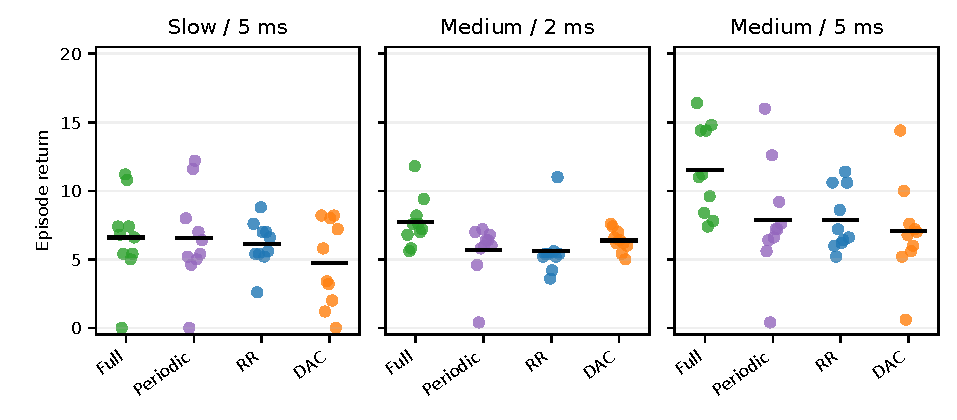
\includegraphics[width=\linewidth]{seed_distribution.pdf}
\caption{Ten independently trained seed means for each of Full, Periodic, RR and DAC in each matched condition; horizontal marks show the mean. Episode repetitions are not independent training replicates.}
\label{fig:seed_distribution}
\end{figure}
\FloatBarrier
\section{Sender substitutions and shared-history checks}\label{app:robustness}
To test selection at the same delivered packet count, we use the ten primary training seeds separately for RR-trained and DAC-trained weights. At prespecified even timesteps along both policies' trajectories, we enumerate every feasible one- or two-sender fresh-message subset, keeping the pre-decision state, policy weights and packet count fixed. Each branch resumes the original access rule thereafter. The best--worst suffix-return range and best-subset regret are hindsight diagnostics, not evidence of performance achievable by an online scheduler. All 2,654 no-op and 2,654 forced-original-subset checks passed. Both compare the full recorded suffix trace: actions, rewards, termination flags, environment states, delivered sender sets, source timestamps and accounted traffic.
Eligible senders are all five agent IDs, including inactive agents; this diagnostic does not filter them by activity or score. The cloned snapshot is immediately before encoding and gate selection, and $k(x)$ is the factual number of delivered packets at that state (one or two here). Define $\mathcal A_{k(x)}=\{A\subseteq\{0,\ldots,N-1\}:|A|=k(x)\}$, the set of all sender subsets of cardinality $k(x)$. All $\binom{5}{k(x)}$ subsets are enumerated under fixed readiness. Forced selection is applied at both admission calls. Transmitter age resets for the actually forced attempted senders, credit is charged for those attempts, and the RR cursor advances by their count, not by their identities. The original access rule resumes from that changed scheduler state; later history changes are part of the total effect.
Let $R_{t:T}(A)$ denote suffix return after delivering $A$ now and resuming the original access rule.
\begin{align}
 V_x(A)&=R_{t:T}(A),\\
 \mathrm{Range}(x)&=\max_{A\in\mathcal A_{k(x)}}V_x(A)-\min_{A\in\mathcal A_{k(x)}}V_x(A),\\
 \mathrm{Regret}(x)&=\max_{A\in\mathcal A_{k(x)}}V_x(A)-V_x(A_{\rm factual}).
\end{align}
Effect is $100\,\mathbf1[\mathrm{Range}(x)>0]$. Within each training seed we average equally over its sampled states, without an intermediate episode average; the reported mean then weights the ten seeds equally. Longer factual episodes therefore contribute more states within a seed. Every interval in Table~\ref{tab:new_fresh} is the unadjusted descriptive Student-$t$ interval of these ten seed means (9 degrees of freedom), not an interval treating branches as independent observations. Regret uses a hindsight best subset and is not achievable online performance. The weighting analysis below directly compares factual and uniform-subset outcomes at the same received count. Candidate branch counts exclude no-op, forced-original and withholding checks; per-seed denominators accompany the supplementary data.
\begin{table}[htbp]\centering\setlength{\tabcolsep}{3pt}\footnotesize
\caption{Feasible-subset effects on primary checkpoints. Each row uses ten frozen primary training seeds, ten evaluation resets per seed and fixed 0.5 ms readiness; Effect is the seed-mean percentage of sampled states with nonzero best--worst return range, with an unadjusted 95\% t interval.}\label{tab:new_fresh}
\vspace{3mm}
\begin{adjustbox}{max width=\linewidth}\begin{tabular}{lllll}\toprule
Condition & Weights & States & Subsets & Effect (\%) [CI]\\\midrule
Slow/5 ms & RR & 646 & 3,230 & 18.86 [15.33, 22.40]\\
Slow/5 ms & DAC & 687 & 3,435 & 13.94 [9.45, 18.44]\\
Medium/2 ms & RR & 661 & 6,610 & 16.97 [9.99, 23.94]\\
Medium/2 ms & DAC & 660 & 6,600 & 18.16 [11.13, 25.19]\\
\bottomrule\end{tabular}\end{adjustbox}\end{table}
\begin{table}[htbp]\centering\setlength{\tabcolsep}{3pt}\footnotesize
\caption{Shared-prefix effects on frozen primary checkpoints: ten training seeds, 20 resets per seed and fixed 0.5 ms readiness. Both differences are DAC minus RR under the indicated weights; cold starts use empty caches, while prefix branches share an RR initialization. Early termination is retained; intervals use ten seed means.}\label{tab:new_prefix}
\begin{adjustbox}{max width=\linewidth}\begin{tabular}{lllll}\toprule
Condition & Weights & Cold diff. & Prefix diff. [95\% CI] & Survivors\\\midrule
Slow/5 ms & RR & -0.850 & +0.000 [0.000,0.000] & 183/200\\
Slow/5 ms & DAC & +0.200 & +0.000 [0.000,0.000] & 190/200\\
Medium/2 ms & RR & -1.700 & +0.350 [-0.235,0.935] & 199/200\\
Medium/2 ms & DAC & -0.200 & -0.350 [-1.025,0.325] & 200/200\\
\bottomrule\end{tabular}\end{adjustbox}\end{table}
Define the paired factual-minus-uniform contrast at state $x$ as
\[
\Delta_x=V_x(A_{\rm factual})-|\mathcal A_{k(x)}|^{-1}\sum_{A\in\mathcal A_{k(x)}}V_x(A).
\]
This enumerates a one-decision uniform reference, not a trained random scheduler. Equal-state weighting averages states within each seed; equal-episode weighting first averages states within episodes, then episodes within seeds. Both weight ten seeds equally; intervals use unadjusted Student-t inference with 9 degrees of freedom. Empty strata are not zero-imputed. Table~\ref{tab:robust_strata} shows the change of estimand explicitly. The 224 sampled states with no unresolved group have zero range. No factual episode incurred the simultaneous-arrival penalty. One of 19,875 saved counterfactual suffix totals is negative; nonnegative totals can still conceal intermediate penalties, so these checks do not remove all dependence on Hallway's transition rules.

\begin{table}[htbp]\centering\setlength{\tabcolsep}{3pt}\footnotesize
\caption{Fresh-subset sensitivity. Effect columns are percentages: original equal-state weighting, equal-episode weighting, and equal-state weighting restricted to unresolved tasks. All three weight seeds equally. Direct factual minus uniform-subset suffix return uses the identical sampled state and received count; unadjusted 95\% t intervals over ten seeds. Episode weighting first averages sampled states within an episode.}\label{tab:robust_strata}
\begin{adjustbox}{max width=\linewidth}\begin{tabular}{lllllll}\toprule
Condition & Weights & State & Episode & Unresolved & Paired state [CI] & Paired episode [CI]\\\midrule
Slow/5 ms & RR & 18.86 & 21.79 & 24.19 & -0.056 [-0.277, 0.166] & -0.178 [-0.526, 0.171]\\
Slow/5 ms & DAC & 13.94 & 14.76 & 16.48 & 0.182 [0.008, 0.356] & 0.130 [-0.064, 0.324]\\
Medium/2 ms & RR & 16.97 & 19.14 & 25.92 & 0.235 [0.100, 0.371] & 0.195 [-0.027, 0.418]\\
Medium/2 ms & DAC & 18.16 & 19.48 & 22.21 & -0.145 [-0.439, 0.149] & -0.249 [-0.636, 0.139]\\
\bottomrule\end{tabular}\end{adjustbox}\end{table}

\paragraph{Decision scale}
For an episode drawn from the evaluation resets, the average sampled decision within that episode favors the factual subset over a uniform feasible subset by $+0.130$ return points for Slow/DAC (95\% interval $[-0.064,0.324]$) and $-0.249$ for Medium/DAC ($[-0.636,0.139]$). These are one-decision total effects conditional on the respective policy histories. A future deployment that replaced the scheduler at every step would have a different state distribution and requires its own rollout. The state-weighted best--worst ranges instead ask how often some feasible choice matters, including a hindsight choice unavailable at deployment.

\paragraph{Remaining opportunities}
All 800 common prefixes were replayed. A privileged action reference schedules active groups at distinct feasible arrival times; its predicted reward matches 3,406 executed suffix steps. Slow/5 ms has 65, 296 and 39 endpoints with attainable remaining rewards 0, 10 and 20, respectively; 335 admit more reward than either learned suffix. Medium/2 ms has 1, 260 and 139 such endpoints and 361 with unused opportunity. This action-changing reference tests saturation, not message-only causality.
\FloatBarrier
\section{Broadcast learning and receiver probes}\label{app:probe}
We trained five access conditions (None, Ideal, Periodic, RR and DAC) on five-agent broadcast and XOR using ten seeds per condition. Source 0 observes a fresh signed bit in broadcast. In XOR, sources 0 and 1 observe independent bits. Followers receive no current bit, source action or reward. All agents see normalized time. Reward is the fraction of correct follower predictions per step over a horizon of 20. The mixer sees bits and time during training. The decentralized heads see local input and messages. All 100 runs used Adam ($5\times10^{-4}$), 1,000 updates, a batch of 16, replay capacity 1,000, hidden/message sizes 64/8 and no demonstrations. Training used Medium/2 ms. Final evaluation used Medium/5 ms, Medium/2 ms and Slow/5 ms with 50 paired resets. The ideal-link gate required at least eight of ten seeds to reach 75\% accuracy. With measured readiness on resets 9500000--9500049, ten broadcast seeds passed and no XOR seed passed.

The probe instead fixes readiness at 0.5 ms and uses 20 resets (14200000--14200019). Source-aware access forces source 0 into a subset with the factual delivered count at each cloned state. Source identity is supplied; this is not learned generic selection. The subsequent histories may differ, and equal delivered count does not guarantee equal offered traffic. On all 20 resets, slow-link RR/DAC normal source delivery is 20.0/17.0\%, increasing to 100\% with source-aware access. These original probe rollouts did not measure the additional CPU cost of source-aware selection. The subsequent receiver-adaptation experiment charged this cost, as reported in the main paper.

Episodes 14200000--14200009 fit per-receiver ridge probes~\citep{hoerl1970ridge}; 14200010--14200019 evaluate them and the acting-policy scores in Table~\ref{tab:broadcast_use}. Normalization uses fit episodes only, coefficient $10^{-3}$ and an unpenalized intercept. A pre-hook records the actual 74-dimensional utility-head input; the aggregate is independently reconstructed with validity, decay and self-exclusion. The 40,000 replayed steps preserve source bits, delivery, count and reward; a separate 6,000-step replay checks wire-byte accounting.

Source-aware aggregate-probe minus acting-policy gains are 21.56 [7.19,35.94] and 29.06 [11.90,46.23] percentage points for Slow/5 ms RR and DAC, and 35.74 [23.91,47.57] and 34.91 [19.34,50.49] for Medium/2 ms RR and DAC (unadjusted 95\% t intervals of ten seed means). These probes use training labels unavailable to the acting head. The use of a separate probe follows the distinction between information decodable from fixed features~\citep{alain2016understanding} and behavioral listening~\citep{lowe2019pitfalls}. Decodability rules out absent accessible aggregate information as the sole bottleneck in these cells; it does not identify how to make the policy exploit it.
\begin{table}[htbp]\centering\footnotesize
\caption{Broadcast delivery versus use: fixed 0.5 ms readiness, ten-seed mean accuracy (\%) on the same held-out ten episodes. Normal and source-aware acting policies share weights; the probe is fitted separately on ten disjoint episodes. Source-aware selection preserves the factual delivered count. Paired probe gains are reported in this section.}\label{tab:broadcast_use}
\vspace{3mm}
\begin{adjustbox}{max width=\linewidth}\begin{tabular}{lllll}\toprule
Condition & Weights & Normal policy & Source-aware policy & Source-aware aggregate probe\\\midrule
Slow/5 ms & RR & 51.90 & 78.44 & 100.00\\
Slow/5 ms & DAC & 50.27 & 70.94 & 100.00\\
Medium/2 ms & RR & 54.98 & 64.17 & 99.91\\
Medium/2 ms & DAC & 53.35 & 65.09 & 100.00\\
\bottomrule\end{tabular}\end{adjustbox}\end{table}
\FloatBarrier
\section{SMACv2 learning and replay checks}
We use the procedural SMACv2 benchmark~\citep{ellis2023smacv2}. The initial Ideal Full pilot used three seeds each in Terran and Protoss. Final win rates of 3.125--9.375\% after approximately 100,000 environment steps fell below its preset criterion. A separate Terran continuation passed at 300,000 steps (17/64, 14/64 and 19/64 wins). Independent-engine replay then failed at seed 1 after 320 evaluation episodes, precluding the paired scheduler comparison.

The separate Terran 5v5 smoke checked 20 single-episode cells (1,046 steps) on one seed-0 checkpoint, crossing five deployments, two links and fixed versus measured readiness. With readiness fixed at 0.5 ms in Slow/5 ms, Full and shadow RR matched sender identities, timestamps, caches, recurrent states and actions for all 47 steps. Offered traffic fell from 240 to 48 wire B/step at the same 32 payload B/step. At Medium/2 ms both delivered 64 payload B/step, but Full delivered $\{1,2\}$ and RR $\{2,3\}$ at the second decision. The shadow sees factual environment inputs, so its subsequent trace cannot estimate an independent return. This smoke verifies the instrumentation.

\FloatBarrier
\section{External MNIST-sum learning and paired-result checks}\label{app:external}
In the one-step task of Eccles et al.~\citep{eccles2019biases}, each agent observes a different MNIST digit image~\citep{lecun1998gradient}. The speaker chooses one of 20 discrete messages. The listener observes its own image and the message and chooses among 19 possible sums. Both earn one for the correct sum. Conditioning on the listener's digit alone leaves the speaker's digit unknown. The published comparison therefore provides an external case where communication has decision value, and directly addresses positive listening. Each episode has one sender and no cache history. The same-count sender and shared-prefix controls apply to Hallway, not to this game.

We reconstructed the two convolutional policies and independent REINFORCE updates~\citep{williams1992simple} from the paper and its supplement. Both training arms can send a message. The both-bias arm adds losses that encourage the speaker to condition its symbol on its image and the listener to condition its action on that symbol. The no-bias arm omits these auxiliary objectives. Both-bias and no-bias arms use three matched initialization seeds and the same image-pair streams. The two networks have 32- and 64-channel convolutions with kernel 5, pooling and a 1,024-unit hidden layer. The listener concatenates the one-hot symbol after the convolutional encoder. Adam uses learning rate 0.0003 and batches of 32. Digit labels determine shared reward and offline diagnostic scores. The action and message policies receive images and learn from sampled reward. We use the marginal-entropy coefficient in Eq.~(3) of the original paper, and direct the message-free cross-entropy gradient toward the predictor as in its algorithm. These choices matter because the equation and pseudocode differ in the placement of the entropy coefficient. The release records the reconstruction choices.

The learning criterion requires all three both-bias seeds to exceed 0.20 sampled reward on 1,024 validation pairs and outperform a shuffled speaker on expected reward. The reward threshold follows the published definition of a good run. We reserve 10,000 images from the training split for milestone selection and the official test images for reporting. Both arms are evaluated at the same checkpoints. We stop at the first common milestone that passes using validation data alone. Compared with the original study of 50 runs, the present comparison tests a smaller set of seeds and addresses a delivery intervention.

No seed passed at 3,000 updates, one passed at 6,000 and all three passed at 12,000 (sampled validation reward 0.474, 0.433 and 0.534). We stopped both arms there. On 2,048 held-out pairs per seed, mean sampled test accuracy was 50.21\% with both biases and 9.67\% without them. Eccles et al.~\citep{eccles2019biases} reported 0.98 mean final reward in successful both-bias runs. Our first passing checkpoints establish useful communication at an intermediate level of proficiency.

We froze the three passing policies and used a further 1,024 official-test image pairs per seed. The pairings were distinct from the preceding test. For each pair we summed the model probabilities of a correct answer over all 20 messages and 19 actions. Thus each observation estimates one episode's expected reward under the stochastic policies. Intervals use the three paired seed means on common image pairs and are descriptive. We imposed a 17-byte packet including a 16-byte header, a 100,000 B/s serial link and 50 microseconds of propagation. Preparation took 100, 300, 600 or 900 microseconds, assigned in a balanced order independent of the labels. An omitted or late message produced the same zero-message input. The timing model defines a reception cutoff and assumes preparation times are known to the timing-informed rule.

\paragraph{Paired-result checks}
In MNIST-sum, we reconstructed each pair's probability of a correct answer from the frozen speaker and listener distributions. We then applied the recorded arrival and offer masks and compared the result with the saved reward for each of the 15,360 combinations of image pair, seed and deadline. In Hallway, a branch that repeats the original sender choice must reproduce the factual actions, rewards, termination, sender identities and cache timestamps before an alternative branch can be interpreted. In broadcast, we paired the original and adapted heads by training seed and reset, checked the delivery schedule, and summed the 20 observed rewards in each rollout. This last check measures the outcome after the new head acts and the environment responds.


\FloatBarrier
\bibliographystyle{elsarticle-num}\bibliography{references}
\end{document}
